\documentclass[10pt,a4paper]{article}
\usepackage[margin=17mm]{geometry}
\usepackage[T1]{fontenc}
\usepackage{lmodern}
\usepackage{microtype}
\usepackage{booktabs,tabularx,array}
\usepackage{xcolor}
\usepackage{enumitem}
\usepackage{hyperref}
\usepackage{tikz}
\usepackage{graphicx}
\usetikzlibrary{arrows.meta,shapes.geometric,positioning}

% Paste the shared Colab URLs between the braces, then recompile.
% These fields are intentionally empty. No notebook is publicly hosted yet.
\newcommand{\ResultsURL}{}
\newcommand{\PolicyNotebookURL}{}

\definecolor{ink}{HTML}{15364A}
\definecolor{accent}{HTML}{147D85}
\definecolor{muted}{HTML}{52636C}
\hypersetup{colorlinks=true,urlcolor=accent,pdftitle={An integration law: proposal and ABM evaluation},pdfauthor={ABM course}}
\renewcommand{\familydefault}{\sfdefault}
\setlength{\parindent}{0pt}
\setlength{\parskip}{5pt}
\setlist[itemize]{leftmargin=13pt,nosep,topsep=3pt}
\pagestyle{empty}
\newcommand{\briefhead}[1]{\par\vspace{5pt}{\large\bfseries\color{ink}#1}\par\vspace{1pt}}

\begin{document}
{\small\bfseries\color{accent}1 | INITIAL PROPOSAL \hfill Hypothetical classroom case}
\par\vspace{6pt}
{\LARGE\bfseries\color{ink}Residential Integration Act:\\proposal from the close advisers}
\par\vspace{3pt}
{\color{muted}To the decision maker | For referral to the analytical body | 17 October 2026}

\briefhead{The problem and the political setting}
A dictatorial government's close advisers regard geographically concentrated, racially homogeneous neighborhoods as a potential source of collective mobilization against the regime. They propose residential mixing as a means of reducing that perceived revolt risk. The government controls residential allocation and expects obedience. The advisers' belief about revolt risk is a premise of this proposal, not an established fact.

\textbf{Residential context:} Approximately 85\% of residential locations are occupied, leaving about 15\% vacant.

\briefhead{The proposed law}
\textbf{The imposed same-group minimum is 30\% of occupied immediate-neighbor locations.} Residents below that minimum must relocate to a vacant location; those meeting it remain in place. The rule governs action, regardless of residents' personal feelings.

This regulates a \emph{minimum requirement}, not a maximum actual same-group share: a neighborhood with more than 30\% same-group neighbors remains acceptable. The proposal does not require every neighborhood to contain exactly 30\% of one group.

\briefhead{The intended goals}
\begin{itemize}
\item \textbf{Ultimate political goal:} reduce the perceived risk of revolts and preserve regime stability.
\item \textbf{Intermediate objective:} replace homogeneous residential clusters with broadly mixed neighborhoods.
\item \textbf{Administrative objective:} secure compliance and allow residential arrangements to settle.
\end{itemize}

\briefhead{The advisers' rationale}
Our reasoning has two links: requiring acceptance of mixed neighborhoods should produce residential mixing; that mixing should reduce the perceived risk of collective mobilization against the regime. With two groups of roughly equal size, we expect neighborhoods to become roughly balanced. We assume compliance and available vacancies will allow the city to settle.

\briefhead{Current assumptions}
We invoke other governments' residential allocation practices as a provisional benchmark. Documented comparisons, their outcomes, and their local relevance remain to be established by the analytical body. Our current assumptions are:
\begin{itemize}
\item Requiring residents to accept mixed neighborhoods will produce an integrated city.
\item More mixed neighborhoods will reduce the perceived risk of revolt.
\item A uniform rule is appropriate despite local differences in housing availability.
\item Relocation will bring neighborhoods into conformity with the rule and eventually stop.
\item Administrative compliance will indicate progress toward the intended political goal.
\end{itemize}

\briefhead{The requested next step}
\textbf{Refer this proposal to the analytical body before deciding on adoption.} We request an assessment of whether the proposed rule can produce the residential mixing on which the strategy depends, and what evidence supports the expected political benefit.

The assessment should identify weaknesses in this reasoning and the consequences of implementation. Local evidence on residents' choices, moving burdens, and the claimed relationship between mixing and revolt risk is not yet available.

\vfill
{\footnotesize\color{muted}\textbf{Status of this page.} A fictional advisers' memorandum, not an existing law or an endorsement. Its appeal to practices elsewhere is part of the hypothetical rationale, not a verified account of any government. The next page presents the analytical body's evaluation.}

\newpage
{\small\bfseries\color{accent}2 | POLICY MODEL AND DESIGN \hfill Evidence for the decision}
\par\vspace{5pt}
{\LARGE\bfseries\color{ink}Representing the policy as a model}

\briefhead{Dissect: describe what is happening}
The proposed law requires residents to move if too few of their neighbors belong to their own group. A move changes the neighborhood both where someone leaves and where they arrive. It can therefore bring some residents into conformity with the rule while putting others below the minimum, prompting further moves. We ask whether this process produces mixed neighborhoods and eventually stops. The claimed effect on revolt risk lies outside this analysis.

\briefhead{Discretize: define the agents, arena, states, and rules}
\textbf{A1: citizens} are agents with two owned states: \texttt{group} (0 or 1) and \texttt{requirement-met?} (true or false). Each citizen occupies one residential location and evaluates the group composition of nearby citizens.

\textbf{A2: the city} is the arena, represented by a bounded 51 by 51 grid without wrapping. Each location is vacant or occupied by one citizen, recorded as \texttt{occupied\_lot?}. A neighborhood contains the up to eight surrounding locations; edge and corner locations have fewer neighbors. Only occupied neighbors enter the same-group share.

\textbf{Initialization.} Each location is independently occupied with probability 0.85. Each created citizen receives either group with equal probability. Realized occupancy and group proportions vary between runs. Initial requirements and appearance are evaluated, then the clock is reset.

\textbf{Methods and time.} Citizens \textbf{evaluate} their neighborhood, \textbf{move} to a random vacant location when below the imposed minimum, and \textbf{update} their appearance. All required moves precede reevaluation. One cycle ends with a clock increment and has no assigned calendar duration. Obedience is assumed; meeting the minimum does not signify personal approval.\footnote{The same neighborhood abstraction is implemented with fewer stored attributes: temporary counts use \texttt{let}, and one shared \texttt{neighborhood-counts} reporter supports evaluation and the pooled similarity indicator. This coding simplification preserves the rule and measure.}

\noindent
\begin{minipage}[t]{0.49\linewidth}
\vspace{0pt}\textbf{Policy ontology}\par\smallskip
\centering
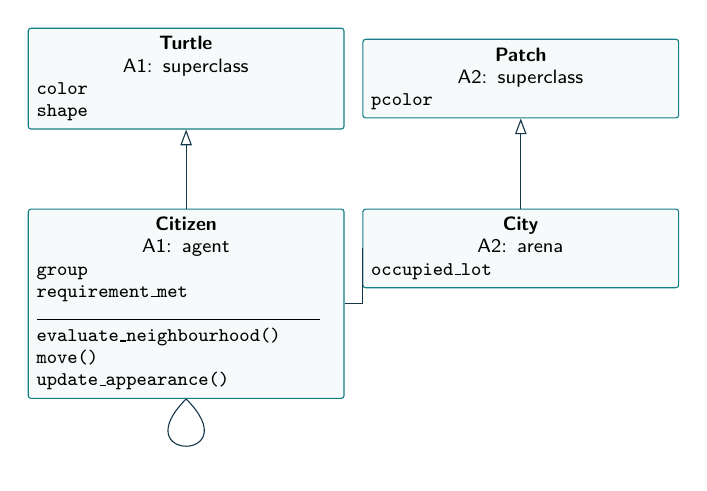
\begin{tikzpicture}[
  cls/.style={draw=accent,rounded corners=1pt,fill=accent!4,text width=38mm,align=left,inner sep=3pt,font=\scriptsize},
  inherit/.style={-{Triangle[open,length=2mm]},draw=ink},
  relation/.style={draw=ink}]
\node[cls] (turtle) at (0,0) {\centering\textbf{Turtle}\par\centering A1: superclass\par\raggedright\texttt{color}\par\texttt{shape}};
\node[cls] (patch) at (4.25,0) {\centering\textbf{Patch}\par\centering A2: superclass\par\raggedright\texttt{pcolor}};
\node[cls,anchor=north] (citizen) at (0,-1.65) {\centering\textbf{Citizen}\par\centering A1: agent\par\raggedright\texttt{group}\par\texttt{requirement\_met}\par\rule{36mm}{0.2pt}\par\texttt{evaluate\_neighbourhood()}\par\texttt{move()}\par\texttt{update\_appearance()}};
\node[cls,anchor=north] (city) at (4.25,-1.65) {\centering\textbf{City}\par\centering A2: arena\par\raggedright\texttt{occupied\_lot}};
\draw[inherit] (citizen.north) -- (turtle.south);
\draw[inherit] (city.north) -- (patch.south);
\draw[relation] (citizen.east) -- (city.west |- citizen.east) -- (city.west);
\draw[relation] (citizen.south) .. controls +(-0.8,-0.8) and +(0.8,-0.8) .. (citizen.south);
\end{tikzpicture}
\par\smallskip\raggedright\footnotesize Classes show owned states, meaningful methods, inheritance, and neighborhood relations.

\end{minipage}\hfill
\begin{minipage}[t]{0.49\linewidth}
\vspace{0pt}\textbf{Policy flowchart}\par\smallskip
\centering
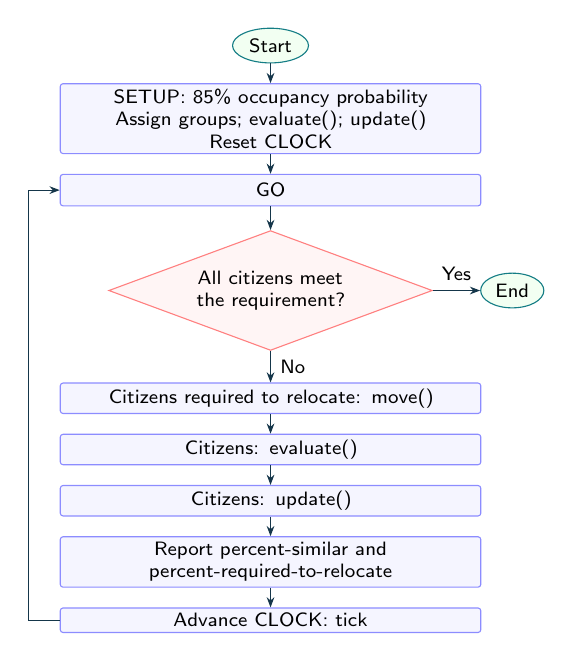
\begin{tikzpicture}[
  processbox/.style={draw=blue!45,fill=blue!4,rounded corners=1pt,text width=52mm,align=center,font=\scriptsize,inner sep=2pt},
  terminal/.style={ellipse,draw=accent,fill=green!5,font=\scriptsize,inner sep=2pt},
  decision/.style={diamond,aspect=2.7,draw=red!50,fill=red!4,text width=25mm,align=center,font=\scriptsize,inner sep=1pt},
  arr/.style={-{Stealth[length=1.3mm]},draw=ink}]
\node[terminal] (start) {Start};
\node[processbox,below=2.5mm of start] (setup) {SETUP: 85\% occupancy probability\par Assign groups; evaluate(); update()\par Reset CLOCK};
\node[processbox,below=2.5mm of setup,minimum height=4mm] (go) {GO};
\node[decision,below=3mm of go] (check) {All citizens meet the requirement?};
\node[terminal,right=6mm of check] (end) {End};
\node[processbox,below=4mm of check] (move) {Citizens required to relocate: move()};
\node[processbox,below=2.5mm of move] (evaluate) {Citizens: evaluate()};
\node[processbox,below=2.5mm of evaluate] (appearance) {Citizens: update()};
\node[processbox,below=2.5mm of appearance] (indicators) {Report percent-similar and\par percent-required-to-relocate};
\node[processbox,below=2.5mm of indicators] (clock) {Advance CLOCK: tick};
\draw[arr] (start.south) -- (setup.north);
\draw[arr] (setup.south) -- (go.north);
\draw[arr] (go.south) -- (check.north);
\draw[arr] (check.east) -- node[above,font=\scriptsize]{Yes} (end.west);
\draw[arr] (check.south) -- node[right,font=\scriptsize]{No} (move.north);
\draw[arr] (move.south) -- (evaluate.north);
\draw[arr] (evaluate.south) -- (appearance.north);
\draw[arr] (appearance.south) -- (indicators.north);
\draw[arr] (indicators.south) -- (clock.north);
\draw[arr] (clock.west) -- ++(-4mm,0) |- (go.west);
\end{tikzpicture}
\par\smallskip\raggedright\footnotesize Indicators are calculated by reporters when requested. This is the simplified cycle diagram; plots update with \texttt{tick}.
\end{minipage}

\briefhead{Implement the given occupancy in setup}
The 85\% value is fixed background information, not an experimental policy input:
\begin{quote}\ttfamily\small
if random 100 < 85 [\quad ; given occupancy probability\\
\hspace*{1em}set occupied\_lot? true\\
\hspace*{1em}sprout-citizens 1 [ ... ]\\
]
\end{quote}
Only the imposed minimum varies between runs; the setup probability remains fixed. At each endpoint, export the summary indicators and citizens' group and coordinates. Notebook 1 analyzes the summary; Notebook 2 uses locations to measure spatial segregation.

\newpage
{\small\bfseries\color{accent}3 | NOTEBOOK 1: EXPERIMENT RESULTS \hfill Evidence for the decision}
\par\vspace{5pt}
{\LARGE\bfseries\color{ink}Does the rule produce mixing that settles?}

\briefhead{What the summary data show}
The summary export contains \textbf{510 runs}: 17 minimums, 10--90\% in five-point steps, with 30 repetitions each. The imposed minimum is the policy input; the final neighbor share is an outcome. They are not the same quantity. A 30\% minimum allows a resident to remain with 30\%, 60\%, or even 100\% same-group neighbors.

\briefhead{How to read the results}
\textbf{Same-group neighbors} describes the share of occupied neighbor links connecting people from the same group. With roughly equal group populations, a value near 50\% is compatible with mixing. \textbf{Still required to move} counts residents below the imposed minimum at the endpoint. \textbf{Settled} means nobody remains below it; it does not mean that neighborhoods are mixed or that residents approve of the policy.

{\small
\begin{tabularx}{\linewidth}{@{}rXXXX@{}}
\toprule
\textbf{Imposed minimum} & \textbf{Same-group neighbors} & \textbf{Still required to move} & \textbf{Median final cycles} & \textbf{Settled runs}\\
\midrule
10\% & 51.3\% & 0\% & 2 & 30/30\\
25\% & 58.9\% & 0\% & 7 & 30/30\\
30\% & 74.1\% & 0\% & 12 & 30/30\\
70\% & 99.7\% & 0\% & 72 & 30/30\\
75\% & 99.9\% & 0\% & 180.5 & 30/30\\
80\% & 51.8\% & 89.0\% & 1,000 (cap) & 0/30\\
90\% & 50.0\% & 98.4\% & 1,000 (cap) & 0/30\\
\bottomrule
\end{tabularx}}
{\footnotesize Selected settings; percentages are means across 30 repetitions. Final cycles at the cap are observation limits, not times to settling.}


\begin{center}
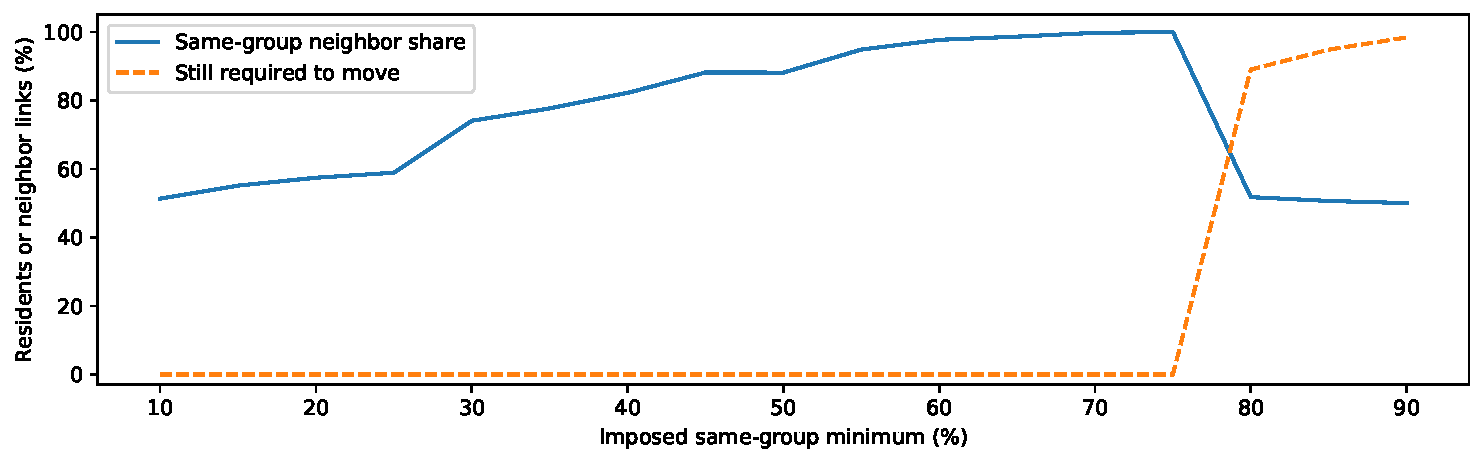
\includegraphics[width=\linewidth]{images/classic_mixing_settling.pdf}
\end{center}
{\footnotesize Figure exported directly from Notebook 1. Means across 30 repetitions at every tested minimum. Lines connect tested settings; they do not establish results between them.}

\briefhead{Policy answer: replace the 30\% proposal}
\textbf{Do not adopt the 30\% minimum as a way to achieve residential mixing.} All 30 runs settle, but same-group neighbor share averages 74.1\%: roughly three out of four occupied neighbor links connect the same group. The rule sets a minimum, not a mixing target; residents can comply while living almost entirely among their own group.

Raising the minimum does not solve this problem. At 70--75\%, similarity approaches 100\% despite every run settling. At 80--90\%, no run settles by the cap; mixed-looking endpoints accompany continuing relocation requirements.

\textbf{Instead, replace the proposed 30\% minimum with a 10\% minimum.} Among the tested settings, it provides the strongest combination of mixing and resolved relocation: all 30 runs settle and mean same-group similarity is 51.3\%. This is the best-supported option among those tested, rather than the only feasible option. Notebook 2 checks this recommendation using spatial segregation measures.

\vfill
{\footnotesize\color{muted}
\textbf{Notebook 1: experiment outcomes.} \ifx\ResultsURL\empty\rule{5cm}{0.3pt}\else\href{\ResultsURL}{Open in Google Colab}\fi\par
The notebook presents means, variation across repetitions, required relocation, and stopping outcomes. Colab URL to be added by the author.
}

\newpage
{\small\bfseries\color{accent}4 | NOTEBOOK 2: SPATIAL ANALYSIS \hfill Evidence for the decision}
\par\vspace{5pt}
{\LARGE\bfseries\color{ink}Go beyond the pooled percentage}

\briefhead{Use locations to measure segregation}
Notebook 1 shows how often immediate neighbors share a group. Here we ask a further question: \textbf{how separated are the groups across local residential areas?} Using saved locations, we count residents in each patch and its up to eight surrounding patches, including vacancies. Boundaries do not wrap.

These areas overlap, like moving a window across a map. Python prepares the spatial table; PySAL calculates the indices. We use the same window in every run. It includes the central patch; the relocation rule counts only surrounding neighbors.

\briefhead{What the three measures mean}
\textbf{Isolation asks: how much does a group mainly encounter itself locally?} A high score means little local exposure to the other group. However, a group that dominates the city naturally encounters itself often, even without residential separation.

\textbf{CorrelationR asks: how much isolation remains after allowing for group composition?} It adjusts for how common the group is in the populations compared. The heatmap compares this adjusted measure with isolation and dissimilarity.\footnote{PySAL first aggregates population within overlapping local environments. CorrelationR is $(I-P)/(1-P)$, where $I$ is isolation and $P$ is the focal-group proportion in those aggregated populations. Small local environments can produce positive scores under random mixing. Scores depend on neighborhood scale; no universal segregation cutoff is applied.}

\textbf{Dissim asks: do the two groups have similar distributions across local areas?} It is low when neighborhood group proportions are similar and high when they differ strongly. These related measures are not independent tests. A score of 0.447 is an index value, \textbf{not a statement that 44.7\% of people are segregated}.

\begin{center}
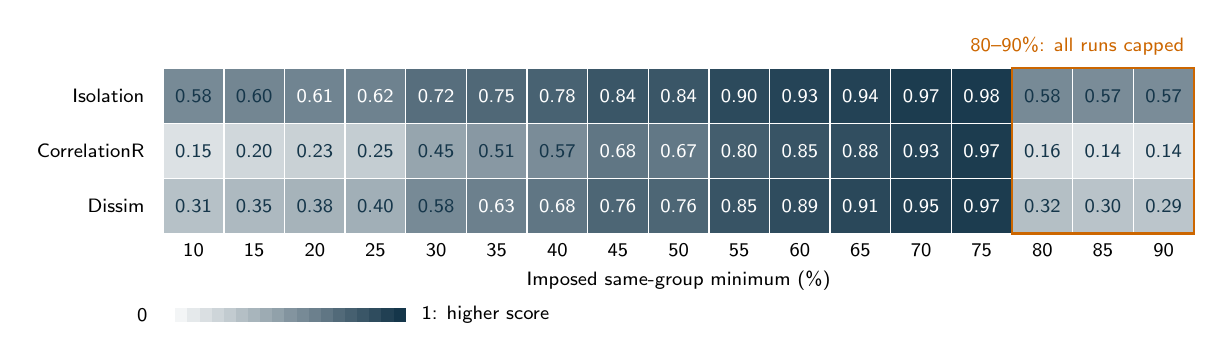
\begin{tikzpicture}[x=0.77cm,y=0.70cm,font=\scriptsize]
\node[anchor=east] at (-0.15,2.5) {Isolation};
\fill[ink!58!white] (0,2) rectangle (1,3);
\draw[white,line width=.5pt] (0,2) rectangle (1,3);
\node[text=ink] at (0.5,2.5) {0.58};
\fill[ink!60!white] (1,2) rectangle (2,3);
\draw[white,line width=.5pt] (1,2) rectangle (2,3);
\node[text=ink] at (1.5,2.5) {0.60};
\fill[ink!61!white] (2,2) rectangle (3,3);
\draw[white,line width=.5pt] (2,2) rectangle (3,3);
\node[text=white] at (2.5,2.5) {0.61};
\fill[ink!62!white] (3,2) rectangle (4,3);
\draw[white,line width=.5pt] (3,2) rectangle (4,3);
\node[text=white] at (3.5,2.5) {0.62};
\fill[ink!72!white] (4,2) rectangle (5,3);
\draw[white,line width=.5pt] (4,2) rectangle (5,3);
\node[text=white] at (4.5,2.5) {0.72};
\fill[ink!75!white] (5,2) rectangle (6,3);
\draw[white,line width=.5pt] (5,2) rectangle (6,3);
\node[text=white] at (5.5,2.5) {0.75};
\fill[ink!78!white] (6,2) rectangle (7,3);
\draw[white,line width=.5pt] (6,2) rectangle (7,3);
\node[text=white] at (6.5,2.5) {0.78};
\fill[ink!84!white] (7,2) rectangle (8,3);
\draw[white,line width=.5pt] (7,2) rectangle (8,3);
\node[text=white] at (7.5,2.5) {0.84};
\fill[ink!84!white] (8,2) rectangle (9,3);
\draw[white,line width=.5pt] (8,2) rectangle (9,3);
\node[text=white] at (8.5,2.5) {0.84};
\fill[ink!90!white] (9,2) rectangle (10,3);
\draw[white,line width=.5pt] (9,2) rectangle (10,3);
\node[text=white] at (9.5,2.5) {0.90};
\fill[ink!93!white] (10,2) rectangle (11,3);
\draw[white,line width=.5pt] (10,2) rectangle (11,3);
\node[text=white] at (10.5,2.5) {0.93};
\fill[ink!94!white] (11,2) rectangle (12,3);
\draw[white,line width=.5pt] (11,2) rectangle (12,3);
\node[text=white] at (11.5,2.5) {0.94};
\fill[ink!97!white] (12,2) rectangle (13,3);
\draw[white,line width=.5pt] (12,2) rectangle (13,3);
\node[text=white] at (12.5,2.5) {0.97};
\fill[ink!98!white] (13,2) rectangle (14,3);
\draw[white,line width=.5pt] (13,2) rectangle (14,3);
\node[text=white] at (13.5,2.5) {0.98};
\fill[ink!58!white] (14,2) rectangle (15,3);
\draw[white,line width=.5pt] (14,2) rectangle (15,3);
\node[text=ink] at (14.5,2.5) {0.58};
\fill[ink!57!white] (15,2) rectangle (16,3);
\draw[white,line width=.5pt] (15,2) rectangle (16,3);
\node[text=ink] at (15.5,2.5) {0.57};
\fill[ink!57!white] (16,2) rectangle (17,3);
\draw[white,line width=.5pt] (16,2) rectangle (17,3);
\node[text=ink] at (16.5,2.5) {0.57};
\node[anchor=east] at (-0.15,1.5) {CorrelationR};
\fill[ink!15!white] (0,1) rectangle (1,2);
\draw[white,line width=.5pt] (0,1) rectangle (1,2);
\node[text=ink] at (0.5,1.5) {0.15};
\fill[ink!20!white] (1,1) rectangle (2,2);
\draw[white,line width=.5pt] (1,1) rectangle (2,2);
\node[text=ink] at (1.5,1.5) {0.20};
\fill[ink!23!white] (2,1) rectangle (3,2);
\draw[white,line width=.5pt] (2,1) rectangle (3,2);
\node[text=ink] at (2.5,1.5) {0.23};
\fill[ink!25!white] (3,1) rectangle (4,2);
\draw[white,line width=.5pt] (3,1) rectangle (4,2);
\node[text=ink] at (3.5,1.5) {0.25};
\fill[ink!45!white] (4,1) rectangle (5,2);
\draw[white,line width=.5pt] (4,1) rectangle (5,2);
\node[text=ink] at (4.5,1.5) {0.45};
\fill[ink!51!white] (5,1) rectangle (6,2);
\draw[white,line width=.5pt] (5,1) rectangle (6,2);
\node[text=ink] at (5.5,1.5) {0.51};
\fill[ink!57!white] (6,1) rectangle (7,2);
\draw[white,line width=.5pt] (6,1) rectangle (7,2);
\node[text=ink] at (6.5,1.5) {0.57};
\fill[ink!68!white] (7,1) rectangle (8,2);
\draw[white,line width=.5pt] (7,1) rectangle (8,2);
\node[text=white] at (7.5,1.5) {0.68};
\fill[ink!67!white] (8,1) rectangle (9,2);
\draw[white,line width=.5pt] (8,1) rectangle (9,2);
\node[text=white] at (8.5,1.5) {0.67};
\fill[ink!80!white] (9,1) rectangle (10,2);
\draw[white,line width=.5pt] (9,1) rectangle (10,2);
\node[text=white] at (9.5,1.5) {0.80};
\fill[ink!85!white] (10,1) rectangle (11,2);
\draw[white,line width=.5pt] (10,1) rectangle (11,2);
\node[text=white] at (10.5,1.5) {0.85};
\fill[ink!88!white] (11,1) rectangle (12,2);
\draw[white,line width=.5pt] (11,1) rectangle (12,2);
\node[text=white] at (11.5,1.5) {0.88};
\fill[ink!93!white] (12,1) rectangle (13,2);
\draw[white,line width=.5pt] (12,1) rectangle (13,2);
\node[text=white] at (12.5,1.5) {0.93};
\fill[ink!97!white] (13,1) rectangle (14,2);
\draw[white,line width=.5pt] (13,1) rectangle (14,2);
\node[text=white] at (13.5,1.5) {0.97};
\fill[ink!16!white] (14,1) rectangle (15,2);
\draw[white,line width=.5pt] (14,1) rectangle (15,2);
\node[text=ink] at (14.5,1.5) {0.16};
\fill[ink!14!white] (15,1) rectangle (16,2);
\draw[white,line width=.5pt] (15,1) rectangle (16,2);
\node[text=ink] at (15.5,1.5) {0.14};
\fill[ink!14!white] (16,1) rectangle (17,2);
\draw[white,line width=.5pt] (16,1) rectangle (17,2);
\node[text=ink] at (16.5,1.5) {0.14};
\node[anchor=east] at (-0.15,0.5) {Dissim};
\fill[ink!31!white] (0,0) rectangle (1,1);
\draw[white,line width=.5pt] (0,0) rectangle (1,1);
\node[text=ink] at (0.5,0.5) {0.31};
\fill[ink!35!white] (1,0) rectangle (2,1);
\draw[white,line width=.5pt] (1,0) rectangle (2,1);
\node[text=ink] at (1.5,0.5) {0.35};
\fill[ink!38!white] (2,0) rectangle (3,1);
\draw[white,line width=.5pt] (2,0) rectangle (3,1);
\node[text=ink] at (2.5,0.5) {0.38};
\fill[ink!40!white] (3,0) rectangle (4,1);
\draw[white,line width=.5pt] (3,0) rectangle (4,1);
\node[text=ink] at (3.5,0.5) {0.40};
\fill[ink!58!white] (4,0) rectangle (5,1);
\draw[white,line width=.5pt] (4,0) rectangle (5,1);
\node[text=ink] at (4.5,0.5) {0.58};
\fill[ink!63!white] (5,0) rectangle (6,1);
\draw[white,line width=.5pt] (5,0) rectangle (6,1);
\node[text=white] at (5.5,0.5) {0.63};
\fill[ink!68!white] (6,0) rectangle (7,1);
\draw[white,line width=.5pt] (6,0) rectangle (7,1);
\node[text=white] at (6.5,0.5) {0.68};
\fill[ink!76!white] (7,0) rectangle (8,1);
\draw[white,line width=.5pt] (7,0) rectangle (8,1);
\node[text=white] at (7.5,0.5) {0.76};
\fill[ink!76!white] (8,0) rectangle (9,1);
\draw[white,line width=.5pt] (8,0) rectangle (9,1);
\node[text=white] at (8.5,0.5) {0.76};
\fill[ink!85!white] (9,0) rectangle (10,1);
\draw[white,line width=.5pt] (9,0) rectangle (10,1);
\node[text=white] at (9.5,0.5) {0.85};
\fill[ink!89!white] (10,0) rectangle (11,1);
\draw[white,line width=.5pt] (10,0) rectangle (11,1);
\node[text=white] at (10.5,0.5) {0.89};
\fill[ink!91!white] (11,0) rectangle (12,1);
\draw[white,line width=.5pt] (11,0) rectangle (12,1);
\node[text=white] at (11.5,0.5) {0.91};
\fill[ink!95!white] (12,0) rectangle (13,1);
\draw[white,line width=.5pt] (12,0) rectangle (13,1);
\node[text=white] at (12.5,0.5) {0.95};
\fill[ink!97!white] (13,0) rectangle (14,1);
\draw[white,line width=.5pt] (13,0) rectangle (14,1);
\node[text=white] at (13.5,0.5) {0.97};
\fill[ink!32!white] (14,0) rectangle (15,1);
\draw[white,line width=.5pt] (14,0) rectangle (15,1);
\node[text=ink] at (14.5,0.5) {0.32};
\fill[ink!30!white] (15,0) rectangle (16,1);
\draw[white,line width=.5pt] (15,0) rectangle (16,1);
\node[text=ink] at (15.5,0.5) {0.30};
\fill[ink!29!white] (16,0) rectangle (17,1);
\draw[white,line width=.5pt] (16,0) rectangle (17,1);
\node[text=ink] at (16.5,0.5) {0.29};
\node at (0.5,-.3) {10};
\node at (1.5,-.3) {15};
\node at (2.5,-.3) {20};
\node at (3.5,-.3) {25};
\node at (4.5,-.3) {30};
\node at (5.5,-.3) {35};
\node at (6.5,-.3) {40};
\node at (7.5,-.3) {45};
\node at (8.5,-.3) {50};
\node at (9.5,-.3) {55};
\node at (10.5,-.3) {60};
\node at (11.5,-.3) {65};
\node at (12.5,-.3) {70};
\node at (13.5,-.3) {75};
\node at (14.5,-.3) {80};
\node at (15.5,-.3) {85};
\node at (16.5,-.3) {90};
\node at (8.5,-.85) {Imposed same-group minimum (\%)};
\draw[orange!80!black,thick] (14,0) rectangle (17,3);
\node[anchor=east,text=orange!80!black] at (17,3.4) {80--90\%: all runs capped};
\fill[ink!0!white] (0.0,-1.6) rectangle (0.2,-1.35);
\fill[ink!5!white] (0.2,-1.6) rectangle (0.4,-1.35);
\fill[ink!11!white] (0.4,-1.6) rectangle (0.6000000000000001,-1.35);
\fill[ink!16!white] (0.6000000000000001,-1.6) rectangle (0.8,-1.35);
\fill[ink!21!white] (0.8,-1.6) rectangle (1.0,-1.35);
\fill[ink!26!white] (1.0,-1.6) rectangle (1.2000000000000002,-1.35);
\fill[ink!32!white] (1.2000000000000002,-1.6) rectangle (1.4000000000000001,-1.35);
\fill[ink!37!white] (1.4000000000000001,-1.6) rectangle (1.6,-1.35);
\fill[ink!42!white] (1.6,-1.6) rectangle (1.8,-1.35);
\fill[ink!47!white] (1.8,-1.6) rectangle (2.0,-1.35);
\fill[ink!53!white] (2.0,-1.6) rectangle (2.2,-1.35);
\fill[ink!58!white] (2.2,-1.6) rectangle (2.4000000000000004,-1.35);
\fill[ink!63!white] (2.4000000000000004,-1.6) rectangle (2.6,-1.35);
\fill[ink!68!white] (2.6,-1.6) rectangle (2.8000000000000003,-1.35);
\fill[ink!74!white] (2.8000000000000003,-1.6) rectangle (3.0,-1.35);
\fill[ink!79!white] (3.0,-1.6) rectangle (3.2,-1.35);
\fill[ink!84!white] (3.2,-1.6) rectangle (3.4000000000000004,-1.35);
\fill[ink!89!white] (3.4000000000000004,-1.6) rectangle (3.6,-1.35);
\fill[ink!95!white] (3.6,-1.6) rectangle (3.8000000000000003,-1.35);
\fill[ink!100!white] (3.8000000000000003,-1.6) rectangle (4.0,-1.35);
\node[anchor=east] at (-.1,-1.48) {0};
\node[anchor=west] at (4.1,-1.48) {1: higher score};
\end{tikzpicture}
\end{center}
{\footnotesize Each cell is a mean across 30 repetitions, rounded to two decimals. Darker cells indicate higher values on a common 0--1 scale; the measures have different meanings and baselines. Orange outlines identify capped endpoints, not settled outcomes.}

\briefhead{Does 30\% avoid segregation? Compare with random mixing}
For each of the 30 endpoints at the proposed minimum, Notebook 2 shuffles group labels 999 times, keeping occupied locations, vacancies, and group totals fixed. It recalculates the same indices with the same neighborhoods. The benchmark is each run's own random-mixing distribution, not a universal segregation cutoff.

{\small
\begin{tabularx}{\linewidth}{@{}lXXX@{}}
\toprule
\textbf{Measure} & \textbf{Proposed 30\%} & \textbf{Random mixing at 30\%} & \textbf{Recommended 10\%}\\
\midrule
Isolation & 0.723 & 0.567 & 0.578\\
CorrelationR & 0.447 & 0.134 & 0.151\\
Dissim & 0.576 & 0.293 & 0.307\\
\bottomrule
\end{tabularx}}
{\footnotesize Means across 30 runs and their shuffled reference arrangements. The 10\% and 30\% settings both settle in all 30 runs.}

\textbf{No: the 30\% rule does not prevent segregation under this benchmark.} In every run, all three scores exceed their random-mixing 95th percentiles; none of the 999 shuffled scores reaches the corresponding observed value. Residents experience excess same-group concentration, it persists after composition adjustment, and the groups are distributed unevenly across local areas. This reinforces Notebook 1: compliance is not integration.

\briefhead{Policy recommendation}
\textbf{Replace the proposed 30\% minimum with 10\%, the best-supported option among those tested.} It resolves relocation while producing lower separation on all three spatial measures. Higher minimums yield stronger separation or unresolved relocation.

The recommendation is to \textbf{reduce segregation, not promise its elimination}. At 10\%, scores still exceed their own random benchmarks in 24/30 runs for Isolation and CorrelationR and 16/30 for Dissim. These simulations support the residential choice between tested rules; they do not establish unique feasibility or the claimed reduction in revolt risk.

\vfill
{\footnotesize\color{muted}
\textbf{Evidence and methods.} Schelling (1969); Wilensky's NetLogo Segregation model (1997), course adaptation by Prof. Jose Magallanes. Data: \texttt{policy-relocation-table.csv} and matching final-position exports; bounded grid, 30 repetitions. PySAL \texttt{segregation} 2.6.0 implements measures based on Massey and Denton (1988): \href{https://pysal.org/segregation/api.html}{methods documentation}. Exact simulation reproduction requires the model and random seeds.\par
\textbf{Notebook 2: spatial segregation.} \ifx\PolicyNotebookURL\empty\rule{5cm}{0.3pt}\else\href{\PolicyNotebookURL}{Open in Google Colab}\fi\par
Colab URLs to be added by the author before public release.
}
\end{document}
